% !TeX root = ../mde-presentation.tex

\section{Authors}  \label{sec:authors}

\begin{frame}{Author}
	\label{frm:author}
	\begin{columns}[T]
		\begin{column}{0.7\linewidth}
			\begin{block}{Philipp S. Sommer}
				Helmholtz Coastal Data Center (HCDC) \\
				Helmholtz-Zentrum hereon GmbH \\
				Max-Planck-Straße 1 \\
				DE - 21502 Geesthacht \\
				\vspace{0.5em}
				\begin{description}
					\item[E-mail] \href{mailto:\authoremail}{\authoremail}
					\item[Telefon] +49 4152 87 2126
					\item[Github] \url{https://github.com/Chilipp}
					\item[Webpage] \url{https://www.philipp-s-sommer.de}
				\end{description}
				\hyperlink{frm:map}{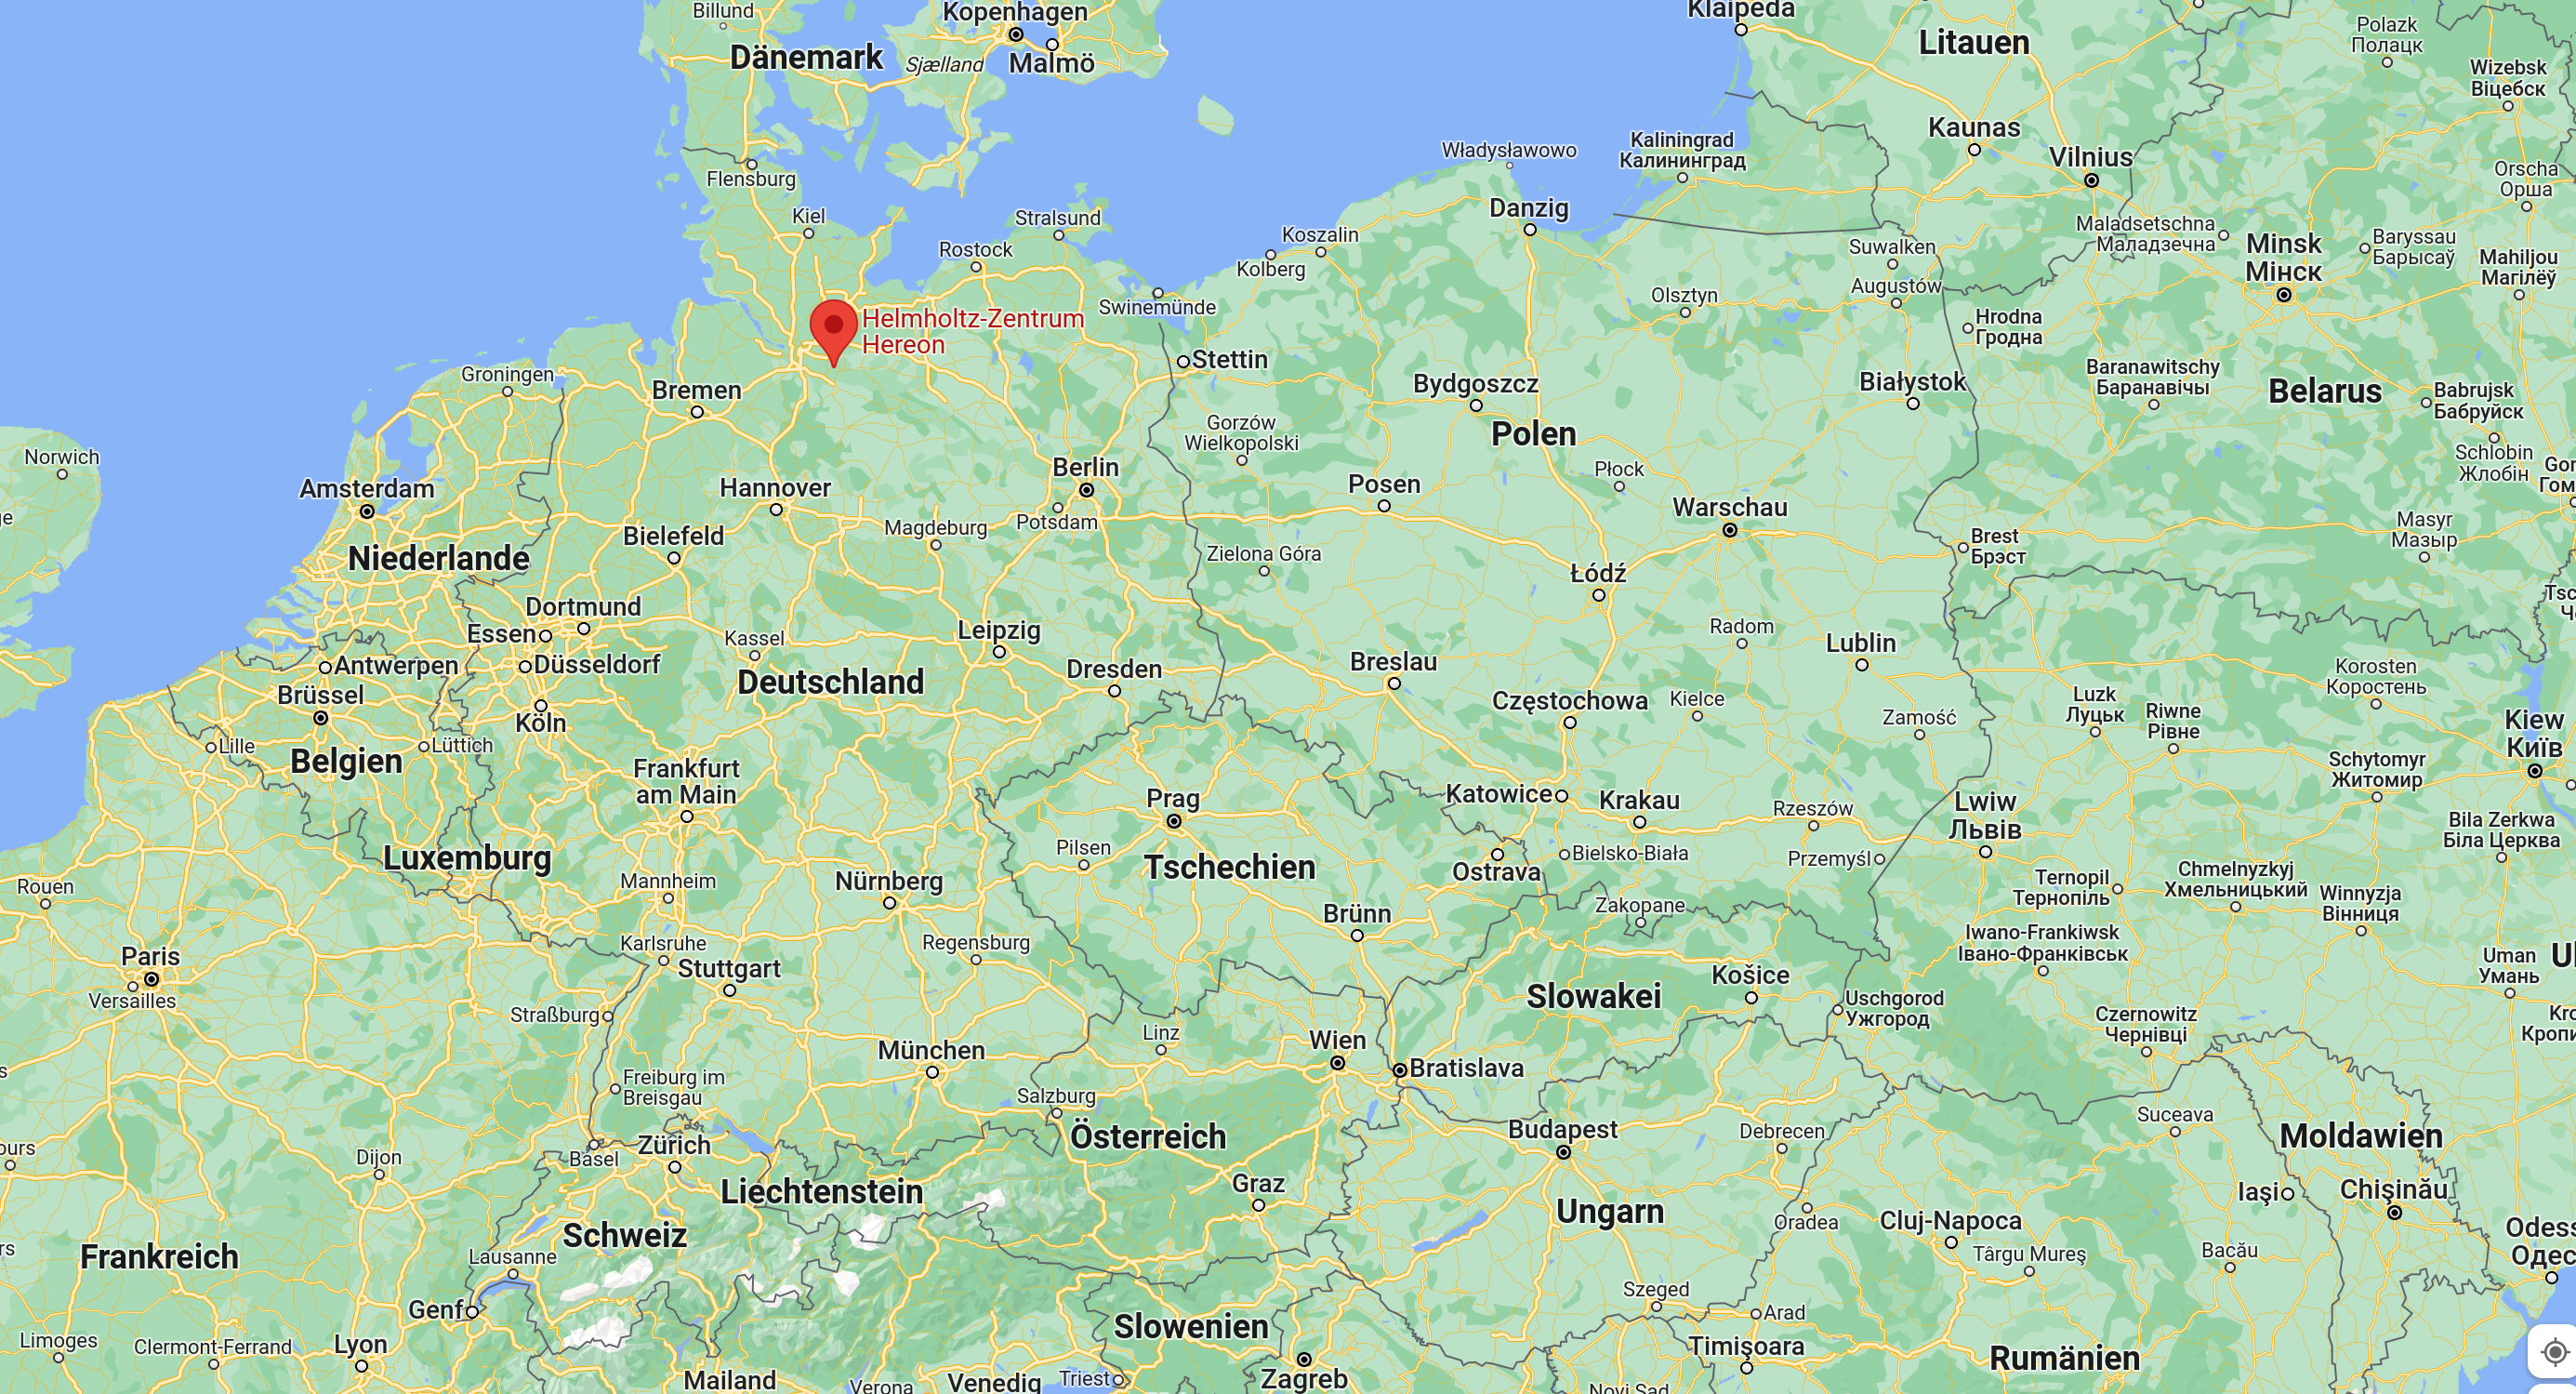
\includegraphics[width=0.25\linewidth]{figures/hereon-map.png}}
			\end{block}
		\end{column}
		\begin{column}{0.25\linewidth}
			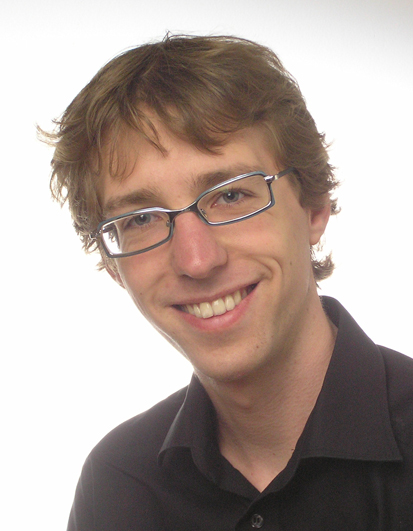
\includegraphics[width=\linewidth]{figures/psommer.jpg}
		\end{column}
	\end{columns}
\end{frame}

\begin{frame}{Co-Authors}

	\begin{columns}[T]
		\begin{column}{0.5\linewidth}

			\begin{block}{Helmholtz-Zentrum Hereon}
				\begin{itemize}
					\item Linda Baldewein
					\item Hatef Takyar
					\item Rehan Chaudhary
					\item Housam Dibeh
					\item Max Böcke
					\item Ulrike Kleeberg
				\end{itemize}
				\vspace{1em}
				\qquad \href{https://www.hereon.de}{
					
\includegraphics[width=0.4\linewidth]{figures/hereon.png}
				}
			\end{block}
		\end{column}

		\begin{column}{0.5\linewidth}
			\begin{block}{Karlsruhe Institute of Technology}
				\begin{itemize}
					\item Mostafa Hadizadeh
					\item Christof Lorenz
				\end{itemize}
			\end{block}

			\begin{block}{Alfred-Wegener-Institut}
				\begin{itemize}
					\item Tilman Dinter
					\item Stefan Pinkernell
				\end{itemize}
			\end{block}

			\begin{block}{Geomar}
				\begin{itemize}
					\item Klaus Getzlaff
				\end{itemize}
			\end{block}

		\end{column}
	\end{columns}

	\vspace{1em}

	\begin{columns}[T]
		\begin{column}{0.3\linewidth}
			\centering
			\href{https://www.awi.de}{
				
\includegraphics[width=0.5\linewidth]{figures/awi_logo.pdf}
			} \\
			\vspace{1em}
			\href{https://www.geomar.de}{
				
\includegraphics[width=0.5\linewidth]{figures/geomar_logo.pdf}
			}
		\end{column}

		\begin{column}{0.3\linewidth}
			\centering
			\href{https://datahub.erde-und-umwelt.de}{
				
\includegraphics[width=0.5\linewidth]{figures/datahub.png}
			 } \\
			\vspace{1em}
			\href{https://www.helmholtz.de/}{
				
\includegraphics[width=0.5\linewidth]{figures/helmholtz.pdf}
			}

		\end{column}

		\begin{column}{0.3\linewidth}
			\centering
			\href{https://kit.edu}{
				
\includegraphics[width=0.5\linewidth]{figures/kit.pdf}
			 } \\
			 \vspace{1em}
			 \href{https://kit.edu}{
				 
\includegraphics[width=0.5\linewidth]{figures/cat4kit.png}
			  }
		\end{column}
	\end{columns}

\end{frame}

\subsection*{Funding} \label{sec:funding}

\begin{frame}{Funding}
	\begin{columns}[T]

		\begin{column}{0.7\linewidth}
			The conceptualization of the Model Data Explorer has been made
			possible through the DataHub funding. Initial developments for
			the THREDDS-Server management are funded through Cat4KIT.

			We hope to get funding through an NFDI4Earth Pilot
			(\url{https://www.nfdi4earth.de/}) for the core implementation
			of the model data explorer.

			\vspace{2.3em}
			\begin{flushright}
				\fcolorbox{hereondarkblueshaded}{white}{
					\begin{tabular}{@{}r@{}}
						\href{https://www.nfdi4earth.de/}{
							
\includegraphics[width=0.4\linewidth]{figures/NFDI4Earth_logo.png}
						} \\
						\textit{\footnotesize *Proposal submitted}
					\end{tabular}
				}
			\end{flushright}
		\end{column}

		\begin{column}{0.3\linewidth}
			\href{https://www.helmholtz.de/}{
				
\includegraphics[width=\linewidth]{figures/helmholtz.pdf}
			} \\
			\vspace{1em}
			\href{https://datahub.erde-und-umwelt.de}{
				
\includegraphics[width=\linewidth]{figures/datahub.png}
			} \\
			\vspace{1em}
			\href{https://kit.edu}{
				
\includegraphics[width=0.5\linewidth]{figures/cat4kit.png}
			}
		\end{column}
	\end{columns}
\end{frame}
